% !TeX root = ../main.tex

\chapter{基于属性的访问控制系统}

\section{系统设计}

\subsection{系统框架}
\begin{figure}
\centering
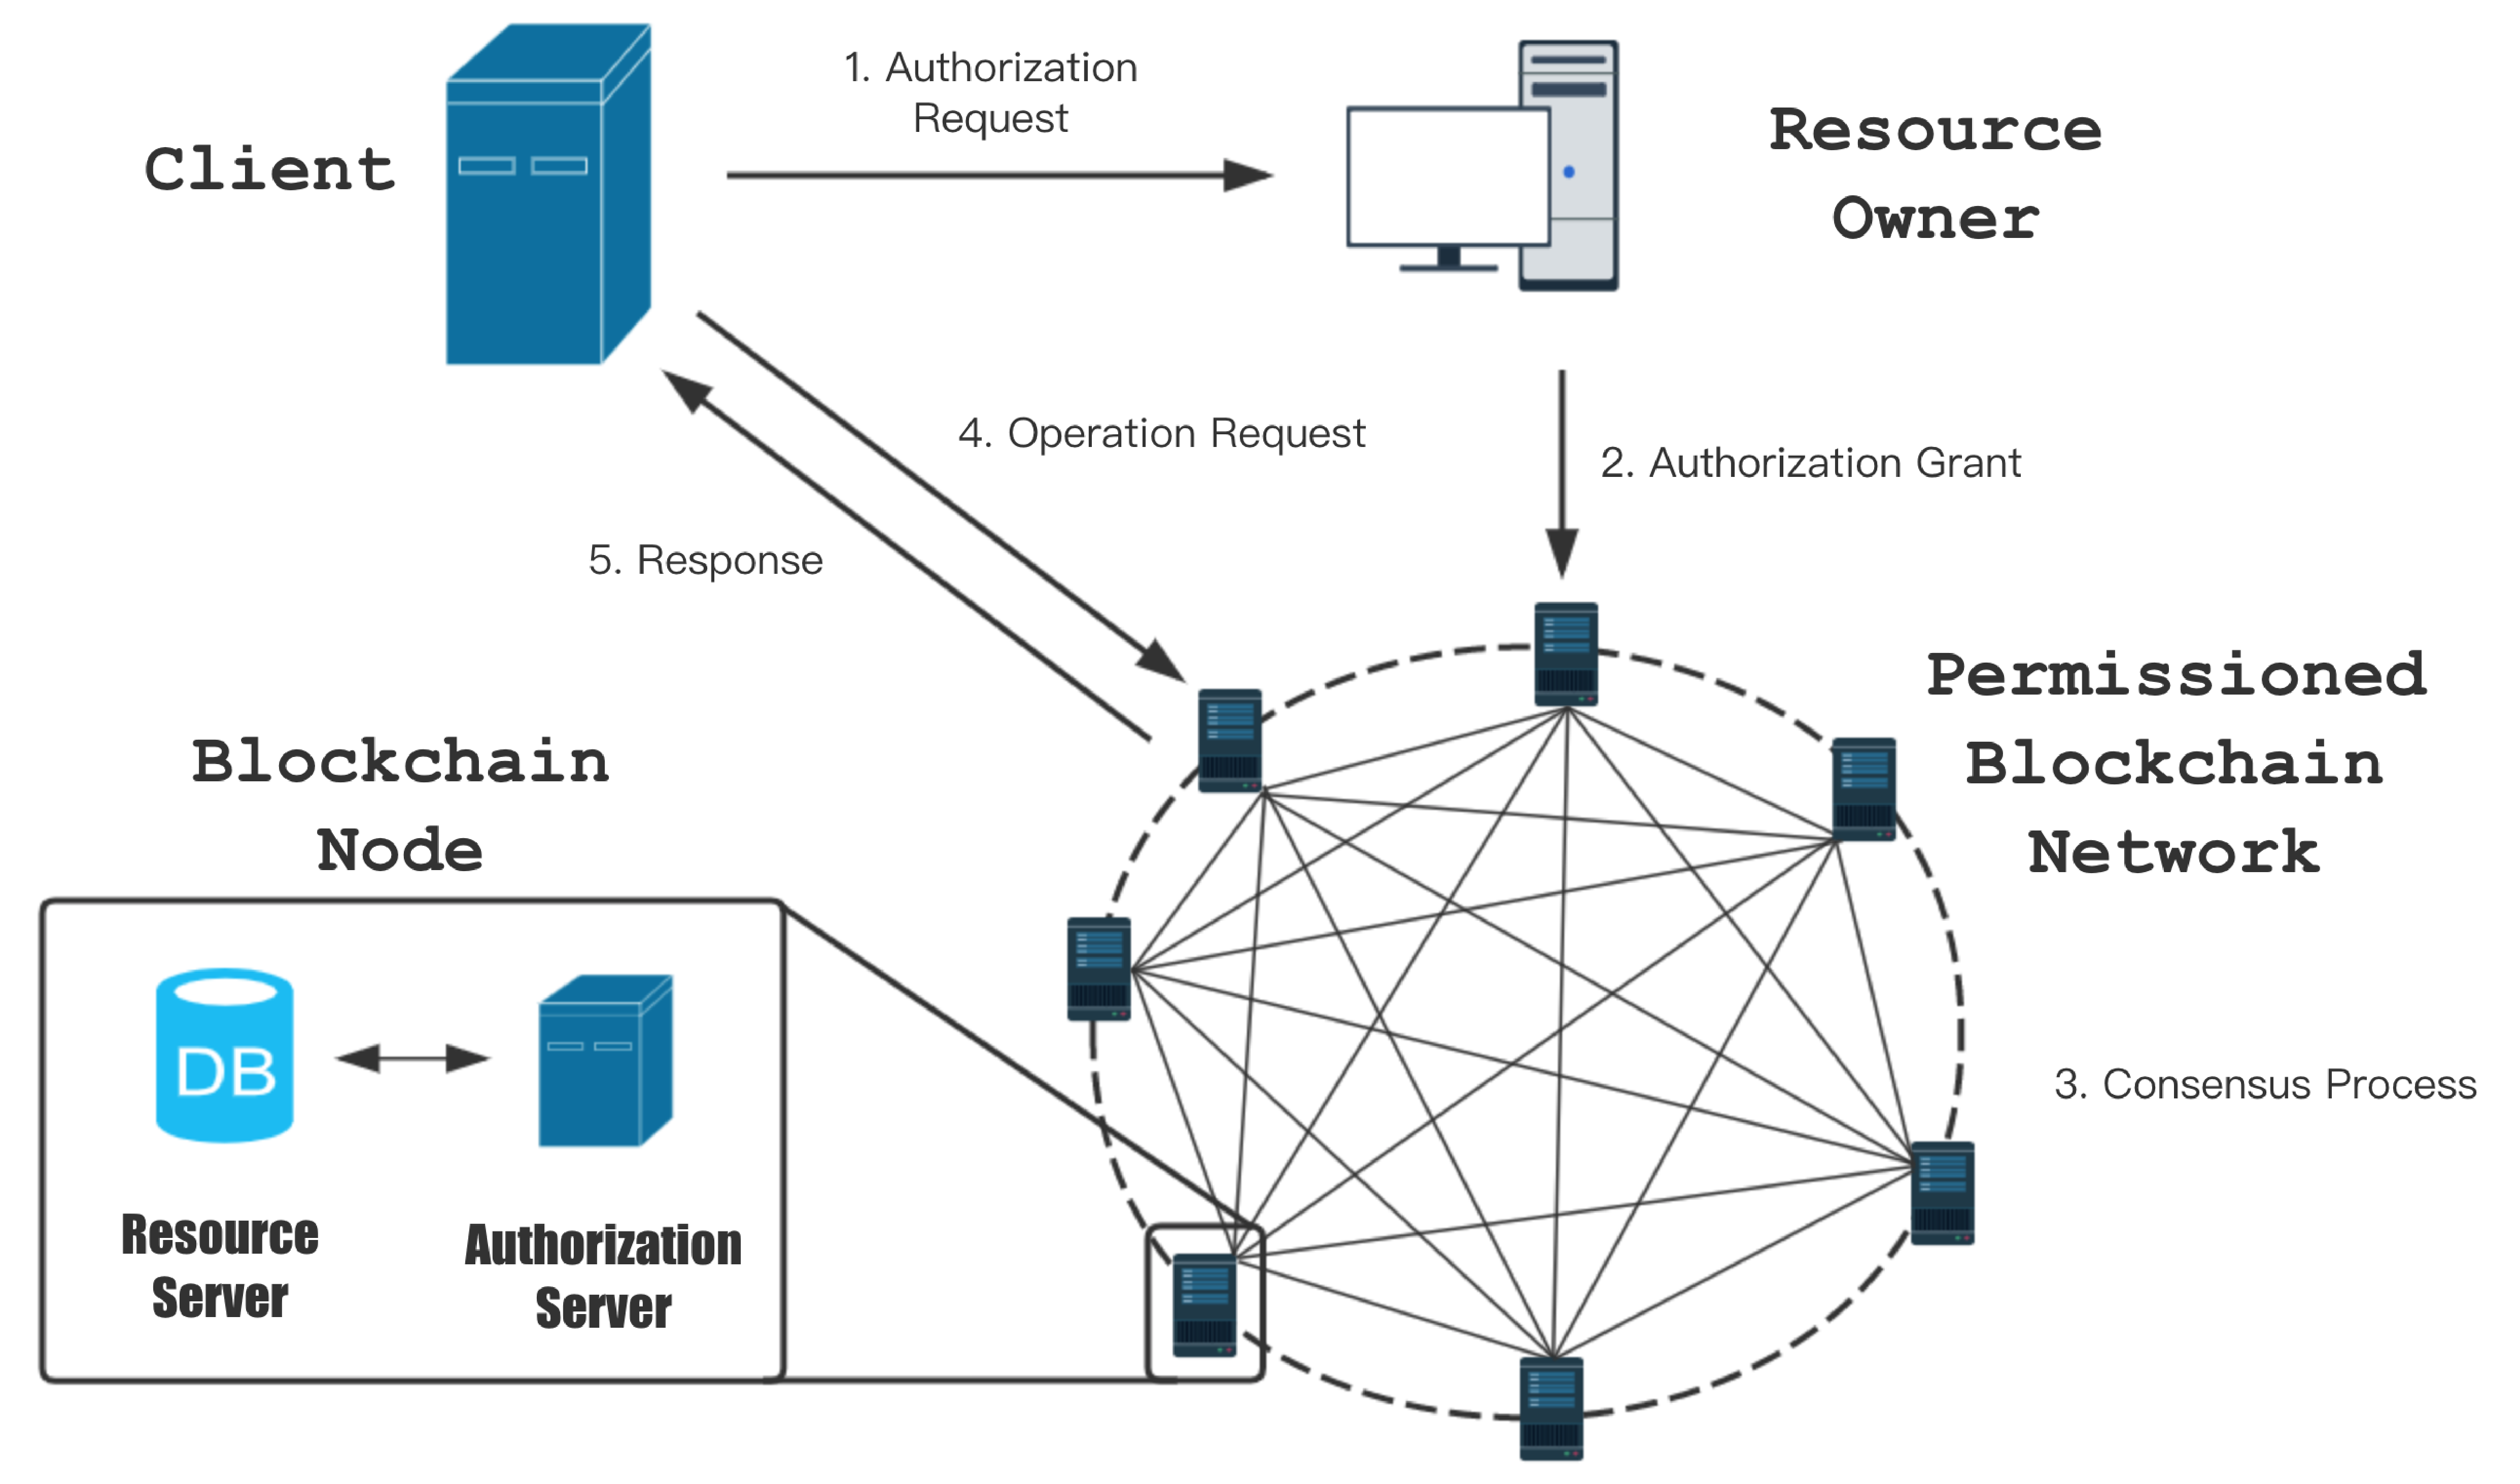
\includegraphics[width=11cm]{figures/archi.eps}
\caption{The Architecture of Decentralized Authorization and Authentication}
\label{fig:framework}
\end{figure}

通过运用区块链技术和基于属性的访问控制模型,我们提出了一个联盟链架构,类似OAuth框架用于第三方授权和认证。图\ref{fig:framework}给出了架构设计和工作流程的概述。该系统包含三类角色,“客户端”作为资源请求者,它请求资源所有者进行授权,并最终请求区块链节点访问资源。“资源所有者”在区块链节点上存储资源,在需要时授予“客户端”访问受保护资源的权限。该架构以联盟网络代替OAuth框架中的中心化认证服务器和资源服务器,该网络中的每个节点具有平等的地位,各自存储用户特定资源并且共同参与用户数据授权和身份验证数据的存储和管理。每个节点由资源服务器和授权服务器组成,其中资源服务器存储用户资源并使用基于属性的访问控制策略进行认证管理。当接收到操作请求时,资源服务器可以使用访问控制策略列表对请求中的各项属性进行身份验证。授权服务器与其他节点的授权服务器共同管理区块链,将用户发起的授权数据存储在区块链中,并且它可以根据区块链对资源服务器提供用于身份验证的各账户的主体属性。

\begin{description}
  \item[\textbf{Client}] The client is the resource requester. It asks the resource owner for authorization and eventually requests the resource server to access the resources needed. Anybody can create an account on-the-fly to play a client role without registration in advance.
  \item[\textbf{Resource Owner}] Resource Owner grants permissions to access protected resources on the resource server. Upon requests, it can authorize the client necessary privileges to execute specific operations on resources.
  \item[\textbf{Blockchain Node}] The consortium blockchain network is comprised of a group of connected nodes. Every node consists of an authorization server and a resource server. The authorization server participates in the distributed consensus process with others to validate the privileges granted by the resource owner, and controls access to the resource server.
\end{description}

该系统在以下几个方面提高了OAuth等中心化访问控制架构的安全性:

\begin{enumerate}
  \item OAuth框架中,第三方平台需要事先在授权服务器进行注册获取客户端密码,然后将客户端密码发送到授权服务器验证身份并获取访问令牌。一旦攻击者入侵了中心化的授权服务器,就可以通过发布伪造的令牌,从而伪装成任何用户访问资源服务器中受保护的资源。该系统中采用的非对称加密系统和去中心化架构可以有效降低攻击的严重程度。在共识达成一致的联盟网络中,攻击者只能访问被入侵的服务器中存储的资源。由于用于电子签名的私钥由用户本地生成并保管,用户发起的操作和授权不能被伪造,从而保护了存储在其他平台上的资源。

  \item 系统中使用的数字签名可以防止跨站请求伪造(Cross-Site Request Forgery,CSRF)攻击。OAuth框架在多个平台广泛实现,并使用重定向URL连接不同的平台,这可能会带来CSRF攻击。例如,它通常用于中心化平台和第三方平台之间的帐户绑定。攻击者可以先访问授权服务器,获得绑定第三方平台和中心化平台账户的访问令牌,然后诱使用户向第三方平台发送绑定请求,并提前提供攻击者获得的令牌。因此,攻击者可以通过中心化平台的账号访问第三方平台上的用户资源。在我们的系统中,用户发送的所有授权和操作都需要进行数字签名,这样才能保证授权的来源。
\end{enumerate}

\subsection{协议流程}
\label{sec:protocols}
本节介绍此框架中的协议。整个协议主要分为5个步骤,分别对应于图\ref{fig:framework}中的工作流程。每一步的详细信息在\ref{sec:protocols}中描述,具体步骤如下:

\begin{enumerate}
  \item 客户端向资源所有者发送$Authorization Request$,其中主要包含客户端的地址和请求授权的属性。
  \item 资源所有者检查$Authorization Request$,如果同意则生成相应的$Authorization Grant$并且发送给任何区块链节点。
  \item 如果接收到的$Authorization Grant$有效,则区块链节点将接受并在网络中传播它。共识过程结束后,授权将被打包到一个新的区块中,并记录到区块链上。
  \item 获得授权后,客户端找到存储需要访问资源的区块链节点,并发送$Operation Request$给该节点的资源服务器。
  \item 资源服务器根据授权服务器提供区块链上账户的主体属性,存储的资源属性以及基于属性的访问控制策略来验证$Operation Request$,根据验证结果回应客户端。
\end{enumerate}

We will describe more details on each step later. There are some basic cryptographic components in our description. Given a message $m$, we define $H(m)$ as the hash of $m$, and $\langle m \rangle_{\sigma_{i}}$ as the message $m$ attached with signature on $H(m)$ from node $i$. This can be used to confirm whether the message has been tampered with during transmission.

Like most blockchain system, to protect the privacy of users, any user can generate accounts freely. The account contains public address and private key $sk$. When the user proposes an authorization or operation, the signature generated from $sk$ will be attached to the message. The signature could be verified using the public key corresponding to the $sk$, which proves the user as the message owner.


\subsection{区块链和属性状态}

Blockchain is the fundamental data structure used in our system to store authorization records. Every node in the network saves a copy of the blockchain. In this system, we adopt account state mechanism from Ethereum project rather than UTXO mechanism in Bitcoin project, because the state design is more suitable for ABAC model. We modify it into the attribute state mechanism in our system. The global state is a set of stats of all accounts. According to the blockchain, we can calculate the state of every account containing the address, the nonce, and the attribute state belonging to the address. The state is saved in memory and can be used to validate authorizations or operations. When appending a new block on the blockchain, the global state changes according to authorizations in the new block. We can regard the global state as the current result of the blockchain. As for the nonce value in the account state, every account has a nonce value which inits as 0. The nonce of address D will increase by one whenever one authorization from address D is recorded on the blockchain. Any authorization with mismatched nonce value will be rejected. This can prevent the replay attack because once the authorization recorded on the blockchain, it cannot be accepted again due to the increased nonce value.

\subsubsection{Authorization verification}
Once the node in the consortium chain network receives the authorization from the client or other nodes, it will first verify the authorization in several aspects. The authenticated authorizations will be added into the authorization pool and wait for packaging into a new block. More details are illustrated in Algorithm \ref{alg:authVerify}.

 \begin{algorithm}
 \floatname{algorithm}{Algorithm}
 \caption{Authorization Verification}\label{alg:authVerify}
   \begin{algorithmic}[!htbp]
   \renewcommand{\algorithmicrequire}{\textbf{Input:}}
   \renewcommand{\algorithmicensure}{\textbf{Output:}}
   \REQUIRE $Authorization$
   \ENSURE  $Verification$
    \STATE $Sender$, $Receiptor$, $Attributes$, $nonce$, $Signature \gets Parse(Authorization)$
    \STATE $AuthorizationHash \gets Hash(Authorizaton)$
    \IF {$CheckSignature(Sender, Hash, Signature) \ne true$}
      \RETURN $false$
    \ENDIF
    \STATE $SenderState \gets GetStateFromAddress(Sender)$
    \IF {$nonce < SenderState.nonce$}
      \RETURN $false$
    \ENDIF
    \FOR {$each Attribute \in Attributes$}
      \IF {$SenderState.VerifyAttribute(Attribute) \ne true$}
        \RETURN $false$
      \ENDIF
    \ENDFOR
    \STATE AddAuthorizationToPool(Authorization)
   \RETURN $true$
   \end{algorithmic}
 \end{algorithm}

\subsubsection{Operation verification}

The resource server synchronizes the blockchain account state and updates the attributes of users. The account state is used as a credential to verify the operation request received from the client. The operation verification process is illustrated in Algorithm \ref{alg:opVerify}.

 \begin{algorithm}
 \floatname{algorithm}{Algorithm}
 \caption{Operation Verification}
   \begin{algorithmic}[H]\label{alg:opVerify}
   \renewcommand{\algorithmicrequire}{\textbf{Input:}}
   \renewcommand{\algorithmicensure}{\textbf{Output:}}
   \REQUIRE $Operation$
   \ENSURE  $Verification$
    \STATE $Sender$, $OpCode$, $Obj$, $nonce$, $Timestamp$, $Signature \gets Parse(Operation)$
    \STATE $OperationHash \gets Hash(Operation)$
    \IF {$CheckSignature(Sender, Hash, Signature) \ne true$}
      \RETURN $false$
    \ENDIF
    \STATE $SenderState \gets GetStateFromAddress(Sender)$
    \IF {$nonce < SenderState.nonce$}
      \RETURN $false$
    \ENDIF
    \STATE$SubAttributes \gets GetAttrFromAddress(Sender)$
    \STATE$ObjAttributes \gets GetAttrFromObject(Obj)$
    \STATE$OpAttributes \gets GetAttrFromOpCode(OpCode)$
    \STATE$EnvAttributes \gets Timestamp$
    \FOR {$each Policy \in Policies do$}
      \IF {$Policy.Match$($SubAttributes$, $ObjAttributes$, $OpAttributes$, $EnvAttributes$) = $true$}
        \RETURN $true$
      \ENDIF
    \ENDFOR
   \RETURN $false$
   \end{algorithmic}
 \end{algorithm}

\subsubsection{Block generation}

The authorizations received by the authorization network will package into a new block at regular intervals. The block interval in the Bitcoin system is 10 minutes, while it is 15 seconds in the Ethereum system. In this system, we set the block interval as 2 seconds, which reduces the latency. The detail of block generation algorithm is shown in Algorithm \ref{alg:blockGeneration}.

 \begin{algorithm}
 \floatname{algorithm}{Algorithm}{}
 \caption{Block Generation}\label{alg:blockGeneration}
   \begin{algorithmic}[!htbp]
   \renewcommand{\algorithmicrequire}{\textbf{Input:}}
   \renewcommand{\algorithmicensure}{\textbf{Output:}}
   \REQUIRE $AuthorizationPool, AUTH\_LIMIT, PreviousBlock$
   \ENSURE  $Verification$
    \STATE $auths \gets ChooseAuths(AuthorizationPool, AUTH\_LIMIT)$
    \STATE $prevHash \gets H(PreviousBlock)$
    \STATE $timestamps \gets CurrentTime()$
    \STATE $newBlock \gets NewBlock(prevHash, auths, timestamps)$
   \RETURN $newBlock$
   \end{algorithmic}
 \end{algorithm}

\subsection{Adapted PBFT Algorithm}

In the traditional distributed consensus domain such as database, researchers have proposed various consensus algorithms to ensure the consistency of data among distributed nodes and provide Byzantine Fault Tolerance (BFT). The Practical Byzantine Fault Tolerance(PBFT) algorithm proposed in 1999 reduces time and communication complexity of BFT, which has been applied on the blockchain system HyperLedger Fabric project. We use a modified PBFT algorithm in the access control system. The nodes in the blockchain network broadcast received requests to others. After a certain period, the master node will package the legal request into blocks. The block is then broadcasted to the network to reach consensus result with other nodes.

\subsubsection{Primary node, backup nodes, and view change}

The design of the primary node, backup nodes, and view change is almost the same as those in PBFT algorithm. The differences are as follow. The primary node in the PBFT algorithm starts consensus process when it receives a request from the client. In this system, the primary node starts consensus every 2 seconds and packages at most 1000 authorizations into a new block. View change happens when backup nodes find that the primary node seems to break down or be hacked. This is the same as view change in PBFT algorithm. Beyond that, when it is long enough, nodes in our system also carry out a view change. This can prevent the black-list attack from the malicious primary node. In the traditional blockchain system, the node generating the new block can select transactions contained in it, thus the malicious node can abandon transactions from accounts in a black list. Recurrent view-changes can prevent black-list attack from a malicious primary node.

\subsubsection{Pre-prepare phase}

When a new block period starts, all nodes go into the pre-prepare phase. In this phase, the primary node selects a list of valid authorizations from the authorization pool, and generates a new block containing authorizations selected. Then, the primary node multicasts the pre-prepare $\langle PRE$-$PREPARE, v, i, block \rangle_{\sigma_{i}}$ to all backup nodes, where $v$ is the view id now, $i$ is the id of the primary node. The creation of $pre$-$prepare$ is shown in Algorithm \ref{alg:preprepareGen}.

 \begin{algorithm}
 \floatname{algorithm}{Algorithm}
 \caption{PRE-PREPARE Generation}\label{alg:preprepareGen}
   \begin{algorithmic}[H]
   \renewcommand{\algorithmicrequire}{\textbf{Input:}}
   \renewcommand{\algorithmicensure}{\textbf{Output:}}
   \REQUIRE $blockchain, authorizationPool, AUTH\_LIMIT,$ $sk, viewID$
   \ENSURE  $pre$-$prepare$
    \STATE $prevBlock \gets blockchain.LastBlock()$
    \STATE $block$ $\gets$ $BlockGenration(prevBlock, AUTH\_LIMIT,$ $authorizationPool)$
    \STATE $pre$-$prepare \gets NewRequest(viewID, block)$
    \STATE $signature \gets sk.Sign(request)$
    \STATE $pre$-$prepare.Signature \gets signature$
   \RETURN $pre$-$prepare$
   \end{algorithmic}
 \end{algorithm}

The verification of $pre$-$prepare$ is illustrated in Algorithm \ref{alg:prepreVerify}. If the verification algorithm returns true, the backup nodes will accept it and enter into prepare phase, otherwise, it will reject the pre-prepare and carry out view change to select another primary node.

 \begin{algorithm}
 \floatname{algorithm}{Algorithm}
 \caption{Pre-Prepare Verification}
   \begin{algorithmic}[H]\label{alg:prepreVerify}
   \renewcommand{\algorithmicrequire}{\textbf{Input:}}
   \renewcommand{\algorithmicensure}{\textbf{Output:}}
   \REQUIRE $pre$-$prepare$, $N$, $ViewID$, $i$, $PkList$
   \ENSURE  $Verification$
    \STATE $viewID$, $nodeID$, $timestamps$, $signature \gets Parse(pre$-$prepare)$
    \IF {$viewID \ne ViewID$}
      \RETURN $false$
    \ENDIF

    \IF {$nodeID \ne ViewID \% N$}
      \RETURN $false$
    \ENDIF

    \STATE $hash \gets H(pre$-$prepare)$
    \IF {$CheckSignature(PkList[i], hash, signature) \ne true$}
      \RETURN $false$
    \ENDIF
   \RETURN $true$
   \end{algorithmic}
 \end{algorithm}

\subsubsection{Prepare phase}

If backup node $i$ accepts a $pre$-$prepare$, it enters into the prepare phase. Node $i$ generates a prepare $\langle PRE$-$PARE, v, i, blockHash\rangle_{\sigma_{i}}$, where $v$ is equal to that in pre-prepare information accepted, $i$ means the node id of the backup node, and $blockHash$ means the hash of block in $pre$-$prepare$. Details are described in Algorithm \ref{alg:prepareGen}. Then the $prepare$ will be multicasted to all other nodes including the primary node. Once a node accepts $2f+1$ prepare messages with the same $v$ and $blockHash$ from different nodes(including the one from itself), it will enter into commit phase.

 \begin{algorithm}
 \floatname{algorithm}{Algorithm}
 \caption{Prepare Generation}
   \begin{algorithmic}[H]\label{alg:prepareGen}
   \renewcommand{\algorithmicrequire}{\textbf{Input:}}
   \renewcommand{\algorithmicensure}{\textbf{Output:}}
   \REQUIRE $pre$-$prepare, nodeID, sk, NeighborList$
   \ENSURE  $prepare$

    \STATE $blockHash$ $\gets$ $H(pre$-$prepare.Block)$

    \STATE $viewID \gets pre$-$prepare.ViewID$
    \STATE $prepare \gets NewPrepare(viewID, nodeID, blockHash)$
    \STATE $signature \gets sk.Sign(prepare)$
    \STATE $prepare.Signature \gets signature$
   \RETURN $prepare$
   \end{algorithmic}
 \end{algorithm}

\subsubsection{Commit phase}

In the commit phase, all nodes in the blockchain network vote for the new block. Node $i$ multicasts a commit $\langle COMMIT, v, i, blockHash \rangle_{\sigma_{i}}$ to other nodes, indicating that it accepts this new block as a consensus result. The commit is generated using Algorithm \ref{alg:commitGen}.

 \begin{algorithm}
 \floatname{algorithm}{Algorithm}
 \caption{Commit Generation}
   \begin{algorithmic}[H]\label{alg:commitGen}
   \renewcommand{\algorithmicrequire}{\textbf{Input:}}
   \renewcommand{\algorithmicensure}{\textbf{Output:}}
   \REQUIRE $prepare, nodeID, blockHash, sk$
   \ENSURE  $commit$

    \STATE $viewID \gets prepare.ViewID$
    \STATE $blockHash \gets prepare.blockHash$
    \STATE $commit \gets NewCommit(viewID, nodeID, blockHash)$
    \STATE $signature \gets sk.Sign(prepare)$
    \STATE $commit.Signature \gets signature$
   \RETURN $commit$
   \end{algorithmic}
 \end{algorithm}

A node accepts a valid commit when receiving it. Once the node accepts $2f+1$ commit messages from different nodes, it makes sure that the new block is committed by at least $f+1$ nodes because there are at most $f$ commits from faulty nodes in the $2f+1$ messages. Then the node enters into the log phase.

\subsubsection{Log phase}

In the log phase, nodes in the authorization network add the new block into blockchain and transmit it to the resource server. Then the resource server updates the state of user accounts according to authorizations in the new block.

\section{原型实现}

\begin{figure}
\centering
\includegraphics[width=12cm, keepaspectratio]{figures/implementation.png}
\caption{The Implementation of Prototype}
\label{fig:implementation}
\end{figure}

We implement a prototype system as shown in Figure \ref{fig:implementation} to verify the feasibility of the designed framework and protocol, and evaluate its performance and latency.

The system is coded in Go programming language. The concurrency primitives(goroutines and channels) in Go language help construct a high-performance network application, which is needed for access control system. The resource server stores protected resources in MongoDB. In the blockchain network, communication among nodes is implemented using HTTP, an application layer protocol based on TCP. This is for rapid development and can be improved in performance by using UDP. On the other hand, HTTPS can be used to enhance the security in the transmission. 

\begin{itemize}
  \item Client: The client is used for users to manage their accounts and keys, authorize other users, and operate resources under their power. The client generates the operations and authorizations and interacts with the servers.
  \item Authorization Server: The authorization server is composed of 4 components:
    \begin{enumerate}
      \item Client Interaction part: this part receives requests from clients and transmits them to solving part.
      \item Blockchain part: this part is connected with other servers, sends and receives blockchain information including operation message, authorization message and block message.
      \item PBFT part: this part sends and receives messages in adapted PBFT protocol. Several timers are designed to guarantee that consensus can be achieved within a limited time period.
      \item Solving part: this part processes messages received from clients or other servers, so it runs generation and verification algorithms described above.
    \end{enumerate}
  \item Resource Server: The resource server is composed of two components:
    \begin{enumerate}
      \item Consensus part: this part validates the consistent results in the blockchain network.
      \item Database part: this part manages the database according to operation request received from clients.
    \end{enumerate}
\end{itemize}

\begin{figure}
\centering
\includegraphics[width=12cm, keepaspectratio]{figures/performance.png}
\caption{Performance Testing}
\label{fig:performance}
\end{figure}

To evaluate the performance of this system, we implement the prototype and deploy 4 blockchain nodes and 1 resource server on the Microsoft Azure cloud platform. Each server is a standard D2s v3 machine, with 2 vCPU, 2G memory, and 1,000 MBps bandwidth.

To test the performance of our system, 1k pairs of keys were generated to simulate 1k users with different attributes, then 10k random authorizations among these users were generated to simulate the authorizations in reality.

The test authorization data is sent to the four nodes at the speed of 500 authorizations per second, and the servers successfully process these requests in about 21 seconds. The distribution of sending time is shown in Fig.\ref{fig:performance}. The servers generat a new block every 2 seconds, and each block contains at most 1000 authorizations (These limitations is set in the code). The authorization number contained in each block is shown in Fig.\ref{fig:performance}. This system reached the performance of about 500 tps(transactions per seconds) on average.